\PassOptionsToPackage{unicode=true}{hyperref} % options for packages loaded elsewhere
\PassOptionsToPackage{hyphens}{url}
%
\documentclass[]{article}
\usepackage{lmodern}
\usepackage{amssymb,amsmath}
\usepackage{ifxetex,ifluatex}
\usepackage{fixltx2e} % provides \textsubscript
\ifnum 0\ifxetex 1\fi\ifluatex 1\fi=0 % if pdftex
  \usepackage[T1]{fontenc}
  \usepackage[utf8]{inputenc}
  \usepackage{textcomp} % provides euro and other symbols
\else % if luatex or xelatex
  \usepackage{unicode-math}
  \defaultfontfeatures{Ligatures=TeX,Scale=MatchLowercase}
\fi
% use upquote if available, for straight quotes in verbatim environments
\IfFileExists{upquote.sty}{\usepackage{upquote}}{}
% use microtype if available
\IfFileExists{microtype.sty}{%
\usepackage[]{microtype}
\UseMicrotypeSet[protrusion]{basicmath} % disable protrusion for tt fonts
}{}
\IfFileExists{parskip.sty}{%
\usepackage{parskip}
}{% else
\setlength{\parindent}{0pt}
\setlength{\parskip}{6pt plus 2pt minus 1pt}
}
\usepackage{hyperref}
\hypersetup{
            pdftitle={Planning for the future: Computing Science and Data Science, an input to the strategic plan of MN-FAK@UiO},
            pdfauthor={Geir Dahl, Ingrid Glad, Morten Hjorth-Jensen, Ole Christian Lingjærde, Heidi Sandaker, Anne H. Schistad Solberg and Geir Olve Storvik},
            pdfborder={0 0 0},
            breaklinks=true}
\urlstyle{same}  % don't use monospace font for urls
\usepackage{longtable,booktabs}
% Fix footnotes in tables (requires footnote package)
\IfFileExists{footnote.sty}{\usepackage{footnote}\makesavenoteenv{longtable}}{}
\usepackage{graphicx,grffile}
\makeatletter
\def\maxwidth{\ifdim\Gin@nat@width>\linewidth\linewidth\else\Gin@nat@width\fi}
\def\maxheight{\ifdim\Gin@nat@height>\textheight\textheight\else\Gin@nat@height\fi}
\makeatother
% Scale images if necessary, so that they will not overflow the page
% margins by default, and it is still possible to overwrite the defaults
% using explicit options in \includegraphics[width, height, ...]{}
\setkeys{Gin}{width=\maxwidth,height=\maxheight,keepaspectratio}
\setlength{\emergencystretch}{3em}  % prevent overfull lines
\providecommand{\tightlist}{%
  \setlength{\itemsep}{0pt}\setlength{\parskip}{0pt}}
\setcounter{secnumdepth}{0}
% Redefines (sub)paragraphs to behave more like sections
\ifx\paragraph\undefined\else
\let\oldparagraph\paragraph
\renewcommand{\paragraph}[1]{\oldparagraph{#1}\mbox{}}
\fi
\ifx\subparagraph\undefined\else
\let\oldsubparagraph\subparagraph
\renewcommand{\subparagraph}[1]{\oldsubparagraph{#1}\mbox{}}
\fi

% set default figure placement to htbp
\makeatletter
\def\fps@figure{htbp}
\makeatother


\title{Planning for the future: Computing Science and Data Science, an input to
the strategic plan of MN-FAK@UiO}
\author{\textbf{Geir Dahl, Ingrid Glad, Morten Hjorth-Jensen, Ole Christian
Lingjærde, Heidi Sandaker, Anne H. Schistad Solberg and Geir Olve
Storvik}}
\date{Oct 30, 2018}

\begin{document}
\maketitle

\hypertarget{executive-summary}{%
\subsubsection{Executive Summary}\label{executive-summary}}

Scientific computing plays a central role in scientific investigations
and is central to innovation in most domains of our lives. It underpins
the majority of today's technological, economic and societal feats. We
have entered an era in which huge amounts of data offer enormous
opportunities, but only to those who are able to harness them.
\href{http://pathways.acm.org/executive-summary.html}{By 2020, it is
also expected that one out of every two jobs in the STEM (Science,
Technology, Engineering and Mathematics) fields will be in computing}
(Association for Computing Machinery, 2013).

Furthermore, the \href{http://www.economist.com/node/21553017}{3rd
Industrial Revolution} will alter significantly the demands on the
workforce. To adapt a highly-qualified workforce to coming challenges
requires strong fundamental bases in STEM fields. Computational Science
can provide such bases at all stages. Most of our students at both the
undergraduate and the graduate level are unprepared to use computational
modeling, data science, and high performance computing -- skills valued
by a very broad range of employers.

These developments, needs and future challenges, will play an essential
role in shaping future technological developments. Most of these
developments require true cross-disciplinary approaches.

This document aims at developing strategies for meeting these future
challenges. One important step in order to meet the future, is the
hiring of new researchers and faculty with the competences and skills
which are needed in order to harness the many new possibilities, as well
as developing new research and educational strategies that can serve our
society at large.

We propose the following: 1. the injection of 15-20 new faculty and
researchers focusing on the science of computational modeling and data
science; 2. the foundation for developing joint cutting-edge graduate
and undergraduate programs in computational science and data science.

\hypertarget{research-and-education-an-outline}{%
\subsubsection{Research and Education, an
outline}\label{research-and-education-an-outline}}

\hypertarget{research}{%
\paragraph{Research}\label{research}}

A central element in addressing the above needs and challenges is the
hiring of new faculty and researchers. We recommend a model where 15-20
new positions (faculty and researchers, permament and/or temporary) are
earmarked for the departments of Mathematics and Informatics in order to
develop new research and educational directions in computational science
and data science.

The new faculty will thus be tasked with developing new research and
educational programs in Computational Science and Data Science. We argue
strongly that the hired faculty can/should have shared positions with
existing departments (for example a 70\% position at say Mathematics or
Informatics and 30\% at the department of Physics), similarly, faculty
with a computational profile and interest at existing departments can
have shared positions at the department of mathematics and informatics.
This will ensure transfer of knowledge as well as the establishment of
new and cross-disciplinary research and oversee the development of new
educational programs and efforts.

These efforts will open doors to new scientific challenges, will enable
UiO to compete and propose new Center-level funding opportunities as
well as totally new research areas (in the Humanities for example) in
computation and data-driven related areas that are currently beyond our
reach. It will facilitate the training of scientists and students to be
an effective 21st century workforce. It will also develop courses on
modern computational techniques and data modeling that meet the needs of
society, both for the public and the private sector.

\hypertarget{education}{%
\paragraph{Education}\label{education}}

We have already developed (started fall 2018) two new Master of Science
programs, one in
\href{http://www.uio.no/english/studies/programmes/computational-science-master/index.html}{Computational
Science} which includes almost all disciplines at the MNFak and one on
\href{http://www.uio.no/english/studies/programmes/datascience-master/index.html}{Data
Science}. These programs form the basis for our educational efforts that
will lead to an \textbf{across the disciplines PhD program} serving the
whole university.

A central aspect is the development and coordination of many of the
educational activities in computational science and data science.

We propose

\begin{enumerate}
\def\labelenumi{\arabic{enumi}.}
\tightlist
\item
  Develop a comprehensive set of courses and degree programs at both
  undergraduate and graduate levels that will give students across the
  university exposure to practical computational methods, understanding
  how to analyse data and more generally to the idea of computers as
  problem-solving tools. The courses and the degree programs can also be
  offered as intensive training courses and programs.\\
\item
  Develop a Bachelor program in Computational Science and Data Science
\item
  Develop an all university PhD program in Computational Science and
  Data Science.
\item
  Based on the new programs (start fall 2018) on Computational Science
  and Data Sciece, Develop an all university Master of Science Program
  in Computational Science and Data Science.
\item
  Develop courses and course modules in Computational Science and Data
  Science for the private and the public sectors.
\item
  Develop a Master of Science program and a PhD program in Computational
  Science and Data Science tailored to the needs of the private and the
  public sectors, allowing for students residing outside UiO to develop
  their knowledge about Computational Science and Data Science.
\item
  Be a driving force in the education of the next generation of school
  teachers and university teachers, with a strong focus on digital
  competences.
\end{enumerate}

\hypertarget{why-should-we-focus-on-computational-and-data-sciences}{%
\subsubsection{Why should we focus on Computational and Data
Sciences?}\label{why-should-we-focus-on-computational-and-data-sciences}}

Modern problems in science and engineering bridge a vast range of
temporal and spatial scales and include a wide variety of physical
processes. The analysis of such problems is not possible, so one must
turn to computation. To develop computational tools for such complex
systems that give physically meaningful insights requires a deep
understanding of approximation theory, high performance computing, and
domain specific knowledge of the area one is modeling. National
laboratories like \href{https://www.simula.no/}{SIMULA research lab}
have addressed the interdisciplinary nature of computing by having
experts in numerical algorithms co-located with disciplinary experts who
have a deep understanding of computation, and who use scientific
computing to address key topics in science.

The proposed organization with algorithmic scientists and disciplinary
scientists in STEM fields as well as other fields is what facilitates
the exploration of challenging multi-disciplinary and interdisciplinary
topics that could not otherwise be addressed. This key observation
motivates the model for the shared positions, with Mathematics and
Informatics as the driving departments.

In addition, the synergy of data-driven computational modeling,
combining aspects of traditional scientific computing with data science
and data mining, is an exciting topic that this new unit will be
uniquely suited to address. This is a rapidly emerging field that
touches many of the STEM disciplines but also Medicine, Education, the
Humanities and the Social Sciences, and attracting world-leading talent
in this area is greatly facilitated by the the above organizational
structure and educational programs.

Furthermore, the development of Computational and Data Sciences has the
potential to catapult UiO into the position of being a leader in this
critical new field, and will open doors to new scientific challenges as
well as new Center-level funding opportunities.

\hypertarget{strengths-possibilities-and-synergies}{%
\paragraph{Strengths, Possibilities and
Synergies}\label{strengths-possibilities-and-synergies}}

The University of Oslo has within several of the STEM fields strong
research and educational activities, exemplified through for example: *
Several Centers of excellence in research where Computational Science
plays a major role * A newly established center of excellence in
education research * Newly established Master of Science programs in
Computational Science and Data Science * Several excellent groups in
STEM fields that do Computational Science and Data Science *
Computational topics are included in all undergraduate STEM programs,
with the possibility to develop a bachelor program in Computational
Science and Data Science for all university colleges * Several
educational prizes and awards related to computational science * Strong
links with research laboratories like SIMULA research lab * UiO has the
potential to develop cross-college educational programs in Computational
Science and Data Science, from undergraduate programs to PhD programs
that serve also the public and the private sectors * The courses to be
developed can be offered to train employees and students outside UiO,
serving thus the coming needs of for example Machine Learning for the
public and the private sectors

With a close coordination between the department of Mathematics and
Informatics, as well as other involved departments, we have the
possibility to really position UiO as the leading Norwegian and perhaps
European institution within Computational Science and Data Science.

\hypertarget{enhance-computational-science-and-data-science-across-the-disciplines}{%
\paragraph{Enhance Computational Science and Data Science across the
disciplines}\label{enhance-computational-science-and-data-science-across-the-disciplines}}

Data driven discovery and data driven modeling play already a central
role in research. The global objective here is to strengthen and
coordinate such activities by bringing together scientists and students
across the disciplines. UiO has already strong computational research
and education activities within Mathematics and the Natural Sciences.
The aim here is to extend this to include

\begin{itemize}
\tightlist
\item
  Computational Science and Data Science in Mathematics and all of the
  physical sciences (Astrophysics, Chemistry, Geoscience and Physics)
\item
  Bioinformatics
\item
  Develop research programs in
  \href{https://www.aps.org/publications/apsnews/201802/ostp.cfm?utm_source=APS+Physics+Main+Group\&utm_campaign=fb7a2e7d6b-News+021218\&utm_medium=email\&utm_term=0_825303224b-fb7a2e7d6b-106513221}{Quantum
  Computing and Quantum Information theory}. Many universities are now
  developing research and
  \href{https://vprgs.msu.edu/event/interdisciplinary-forum-quantum-information-science}{educational
  strategies in Quantum Computing}
\item
  Develop data-driven discovery research programs utilizing recent
  developments in machine learning
\item
  Computational life science
\item
  Computational Materials Science
\item
  Computational Economy and Data Science and computing in Law and the
  Social Sciences
\item
  Data Science and computing in the Humanities
\end{itemize}

The department of Mathematics and Informatics will host and coordinate
research and educational programs in Computational Science and Data
Science. In particular research and education that involve data analysis
and Machine Learning will play a central role here.

\hypertarget{courses-and-degree-programs}{%
\subsubsection{Courses and degree
programs}\label{courses-and-degree-programs}}

Creation of a robust, coherent set of undergraduate and graduate
degrees, with accompanying courses, supports two complementary goals.
First, a coherent program will allow the university to consolidate
undergraduate and graduate training in computation in the STEM fields as
well as introducing computing to other disciplines, reducing redundancy
in the courses taught and allowing the university to offer a wider range
of more specialized advanced courses. Second, we will create a robust
set of degrees that are designed to give our students a strong
introduction to computing that will complement UiO's existing
disciplinary training, and which will make them better suited to be a
part of the workforce in the 21st century, but also to be able to
develop and use computing and data Science across the disciplines. These
programs will include: 1. An undergraduate program in Computational and
Data Sciences tailored to various disciplines. 2. We have already (from
fall 2018) two new Master of Science programs in Computational Science
and Data Science dailored to STEM fields. The aim is to extend these to
other colleges. 3. Develop a cross-college PhD program in Computational
Science and Data Science. 4. Develop courses and course modules in
Computational Science and Data Science for the private and the public
sectors. 5. Develop a Master of Science program and a PhD program in
Computational Science and Data Science tailored to the needs of the
private and the public sectors, allowing for participants residing
outside UiO to develop their knowledge about Computational Science and
Data Science. 6. Be a driving force in the education of the next
generation of school teachers and university teachers, with a strong
focus on digital competences.

This range of options will allow some number of students to dive deeply
into computation through the degree programs, and will enable a much
broader swath of the UiO population to learn about some aspects of
computational and data science through not only the various programs but
also through the courses to be developed by the departments of
Mathematics and Informatics.

One desired result of the creation of these courses and programs is the
foundation of a strong community of students from different disciplines
who use similar techniques to solve a wide range of problems, which will
promote broad, interdisciplinary thinking and will help to raise the
visibility of computing throughout the UiO campus. We note that an extra
benefit of these educational efforts is that UiO will become an ideal
place to perform research in computational science education, a topic of
critical importance that has thus far received little scholarly
attention. The foresee strong links with the recently established Center
for Computing in Science Education.

\hypertarget{long-term-goals-and-sustainability}{%
\paragraph{Long term goals and
sustainability}\label{long-term-goals-and-sustainability}}

The overall goal of this focus on Computational Science and Data Science
is to bring together world-leading faculty who combine the most
important aspects of computation and disciplinary research, thus
enabling cutting-edge interdisciplinary science and the training of both
undergraduate and graduate students. The involved departments will be
economically sustained through the standard base university funding.
However, additional funds will be realized by the securing for example
Center-level funding (as well as many single- or few-PI grants), as well
grants obtained the PIs that sustain graduate students, post-docs,
travel and other associated expenses.

Basic university funding (beyond faculty and support staff salaries) is
necessary to support fellowships for top graduate students, speaker
series and honoraria, visitor support, hardware purchases, and startup
packages.

The enclosed appendices contain more details about research and
education plans. Links to similar and recently established initiatives
are also presented.

\hypertarget{appendix-a-working-group-members-2018}{%
\subsubsection{Appendix A: Working group members (
2018)}\label{appendix-a-working-group-members-2018}}

\begin{enumerate}
\def\labelenumi{\arabic{enumi}.}
\tightlist
\item
  IFI: Ole Christian Lingjærde and Anne H. Schistad Solberg
\item
  Math: Geir Dahl, Ingrid Glad, and Geir Olve Storvik
\item
  Physics: Morten Hjorth-Jensen and Heidi Sandaker
\end{enumerate}

\hypertarget{appendix-b-structure-and-justification-for-planned-organization}{%
\subsubsection{Appendix B: Structure and Justification for Planned
Organization}\label{appendix-b-structure-and-justification-for-planned-organization}}

The joint appointments with other departments will play an important
role in cementing the role of Computational Science and Data Science,
strengthening cross-disciplinarity collaborations. Furthermore, the task
of developing new and joint courses will require extensive
collaborations across departments. As an example, the faculty and
researchers we plan to hire could have a 70\% appointment with the
department of Mathematics or Informatic and 30\% with a single
discipline oriented department. Similarly, a researcher with linked to
the department of Chemistry, could have a shared position of for example
20\% at the Department of Mathematics and 80\% at the department of
Chemistry. These joint appointments will facilitate the seeding of new
research and the development of new courses and degree programs.

One can view the departments of Mathematics and Informatics as hubs
which focus on Algorithms, Computing, Big Data, Mathematics, Quantum
Computing, Machine Learning and Statistical Analysis in close
collaboration with scientists working from the Physical Sciences
(Chemistry, Astrophysics, Physics, Geoscience, Mechanics, Materials
Science), Life Science (Bioscience and Medicine), Law, Education, Social
Sciences and the Humanities. The new department will develop and
strengthen the field of Computational Science and Data Science in close
collaboration with all involved departments (from the MNfak and other
colleges), increasing thereby the overall general competences of our
students and scientific staff on these topics. The following figure
illustrates schematically these links, with the two inner circles
representing the most likely key research activities we wish to
strengthen.

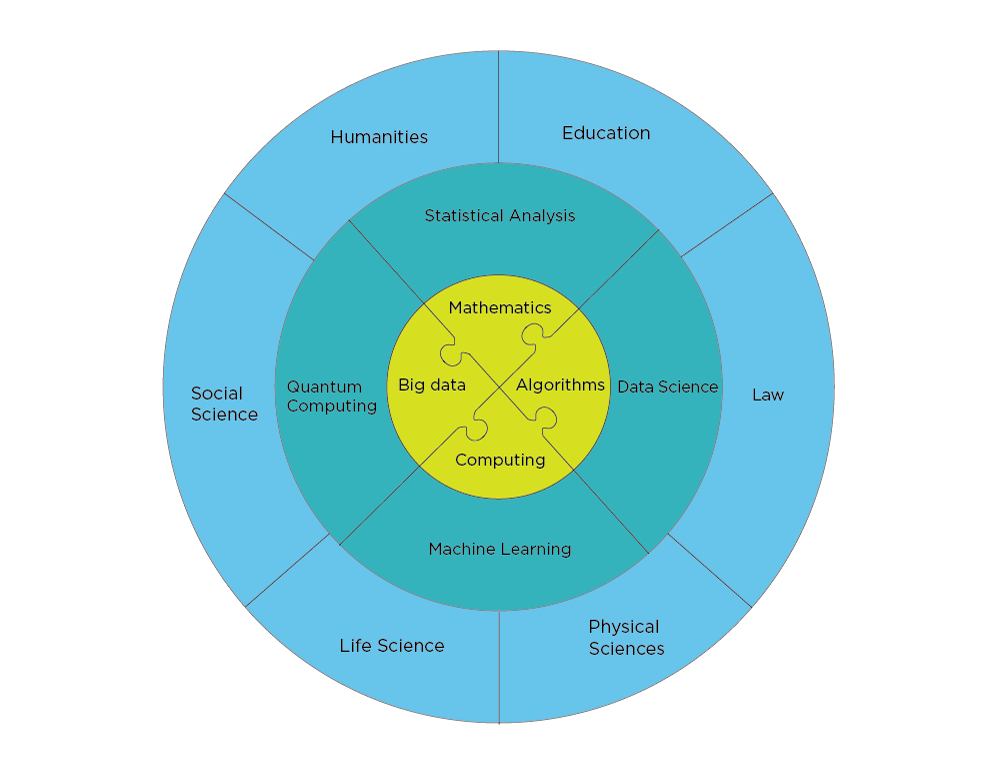
\includegraphics{figslides/topics.png}

\hypertarget{funding}{%
\paragraph{Funding}\label{funding}}

In order to secure funding in addition to those guaranteed by the
University and the ministry of education and research, one should seek
assiduously center funding from the Norwegian SFF and SFI system (under
the auspices of the Research Council of Norway) as well as similar
funding possibilities from the EU. In addition, we expect the faculty to
bring in regular research grants either from industry, the Research
Council of Norway or the EU.

We aim also at exploring and having, out of the 15-20 positions, five
positions at the level of associate or full professor as endowed chairs
and professorships from the private sector. We will in particular target
companies where computational science and data science will play a major
role in the future. The design of research projects linked to the needs
of these companies as well as the PhD and Master of Science programs
discussed below, will make sure that both the private and the public
sector will benefit from highly qualified candidates.

Below we discuss several possible research directions where faculty
hires can start new research directions, in close collaborations with
specialists from various departments.

\hypertarget{appendix-c-sampling-of-new-and-transformational-science-that-can-be-enabled}{%
\subsubsection{Appendix C: Sampling of new and transformational science
that can be
enabled}\label{appendix-c-sampling-of-new-and-transformational-science-that-can-be-enabled}}

There are several new and emerging research directions where
Computational science and Data science will play and can play a major
role.

\hypertarget{computational-life-science}{%
\paragraph{Computational life
science}\label{computational-life-science}}

The Life Sciences is transforming with the explosion of High-throughput
data generation technologies and the need for integrating these across
all the levels of the biological hierarchy. A `system-dynamic' (Systems
Biology) approach will dominate research in the coming decades. Here,
computational modelling to integrate the various data types and data
sets will be a driving force. Similar developments are seen in the field
of molecular image analysis, where computational methods to integrate
the image streams will become essential to make sense of the growing
amount of data. Translational Bioinformatics, bridging the gap between
the laboratory, computer and the clinic, with the ultimate goal of
personalised medicine, is an important, and exciting new dimension. Many
of these developments require cross-disciplinary thinking, and often
breakthroughs in Bioinformatics/Computational Life Science start with
creatively adjusting and implementing algorithmic or computational
solutions originally developed for other fields. A CDS department that
has multidisciplinarity as its founding principle, and brings
computationally skilled researchers from many fields together, will
provide a solid foundation for researchers working towards these
developments.

\hypertarget{develop-data-driven-discovery-research-programs-utilizing-recent-developments-in-machine-learning}{%
\paragraph{Develop data-driven discovery research programs utilizing
recent developments in machine
learning}\label{develop-data-driven-discovery-research-programs-utilizing-recent-developments-in-machine-learning}}

\textbf{Machine Learning} plays nowadays a central role in the analysis
of large data sets in order to extract information about complicated
correlations. This information is often difficult to obtain with
traditional methods. For example, there are about one trillion web
pages; more than one hour of video is uploaded to YouTube every second,
amounting to 10 years of content every day; the genomes of 1000s of
people, each of which has a length of \(3.0\times 10^9\) base pairs,
have been sequenced by various labs and so on. This deluge of data calls
for automated methods of data analysis, which is exactly what machine
learning provides. Developing activities in these frontier computational
technologies is thus of strategic importance for our capability to
address future science problems. The applicability of big data,
data-driven discoveries, data-driven modeling and machine learning
covers basically all disciplines and fields, with applications spanning
from materials science, mechanics, medicine, applied mathematics,
economic forecasting etc. Machine learning and big data concepts are
being exploited in more and more fields. The big data challenge will be
in the forefront of biology and life science research in the next few
years. In materials science machine learning allows us to parametrize
results from quantum mechanical calculations in terms of classical
interactions. These interactions are in turn suitable for large scale
molecular dynamics simulations of complicated systems spanning from
subatomic physics to materials science and life science. To develop a
multiscale science program starting with the smallest constituents and
moving to larger systems can most likely only be done with the
development and application of machine learning algorithms. Economists
and policy makers need up-to-date information on the state of the
economy to formulate effective policies. Variables such as GDP, Gini
factors, unemployment rates, quality of life data etc are normally used
as key indicators. These data are often only available with delays
between collection and availiability to analysts, making it thus
difficult to asses properly their relevance. Machine learning algorithms
have the potential to deliver improved predictions as well as
correlations and proper error estimates. The examples discussed here
represent just a few of the possible applications of Machine Learning
algorithms that the new department can aid in developing. To develop
these research lines will be achieved most effectively within the
multidisciplinary CDS department.

\hypertarget{develop-research-programs-in-quantum-computing-and-quantum-information-theory}{%
\paragraph{Develop research programs in Quantum Computing and Quantum
Information
theory}\label{develop-research-programs-in-quantum-computing-and-quantum-information-theory}}

Enabling simulations of large-scale quantal many-particle systems is a
long-standing problem in scientific computing. Quantum many-particle
interactions define the structure of the universe, from nucleons and
nuclei, to atoms, molecules, and even stars. Since the discovery of
quantum mechanics, a lot of progress has been made in understanding the
dynamics of certain many-particle systems. While some of our insight
comes from a small set of analytically solvable models, numerical
simulations have become a mainstay in our understanding of many-particle
dynamics. The progress in numerical simulations has accelerated in the
last few decades with the advent of modern high performance computing
(HPC) and clever developments in classical simulation algorithms such
as, quantum Monte Carlo,large-scale diagonalization approaches,
Coupled-Cluster theory and other renormalization schemes. Despite the
monumental advances, classical simulation techniques are reaching
fundamental limits in terms of the size of the quantum systems that can
be processed. Fortunately, the disruptive new field of quantum
simulations has emerged, promising to enable simulations far beyond
those which are classically tractable. In particular, scientific
applications concerned with simulations of interacting fermions on a
lattice are poised to reap the benefits of quantum simulations.
Mathematical models of interacting fermions naturally extend to describe
vastly different physics such as that of correlated electronic and the
correlated nuclear systems.

Recent progress in quantum computing as well as digital and analog
Quantum Algorithms (QAs) promise to enable the exciting possibility of
performing simulations that are beyond the reach of all existing and
future classical supercomputers. Despite the progress, there is still a
gap between the resources required by state-of-the-art QA and the
resources offered by available and near-future quantum hardware. It may
take decades of quantum hardware development and engineering before the
current QAs will outperform classical exascale class simulations.
Therefore, to impact scientific computing on a more relevant time scale,
improving the scalability and efficiency of quantum simulation
algorithms is of the highest importance. Developments in quantum
information algorithms and their mathematical properties, as well as
their applications will play a critical role in studies of relevance for
a wide variety of fields, from the design and studies of new materials
to our basic understanding of systems of interest in chemistry and
physics. The new department, in close collaboration with disciplinary
experts, can play an essential role in developing this field by hiring
world-leading experts in quantum information theory and quantum
computing.

\hypertarget{computational-social-science}{%
\paragraph{Computational Social
Science}\label{computational-social-science}}

Survey data, the engine of the behavioral revolution of the social
sciences is about to run its course, with low response rate and poorly
representative samples being the norm rather than the exception.
Fortunately, vast amount of new information from social media, via
digitalized governmental archives, to population registries are opening
up new exiting avenues for innovative social science research, such as
paternity leave and children's performance in school, extent of
censorship in Chinese online new reporting, or conditions for
receptiveness to fake news. Moreover, the new data availability in
combination with tools from machine-learning has spurred an interest in
prediction and sophisticated policy-recommendations, ranging from
optimize relocation of immigrants given their skill-set and local labor
market needs, via probabilistic detection of election fraud, to
forecasting of popular unrest and civil war. The undertaking of such
research questions was, until recently, outside the realm of social
science. There are however limits to the amount of new insights that can
be obtained purely from richer data and ``black-box'' import of
machine-learning tools. More robust, new insights require similar steps
to be taken in the development of applied, testable, theoretical models
to facilitate direct empirical evaluations of the model dynamics and the
consistency of the model with the data. Such a step requires a solid
grounding in computing.

\hypertarget{computational-geoscience}{%
\paragraph{Computational Geoscience}\label{computational-geoscience}}

Geoscience has long been a computationally-intensive area. A typical
climate simulation, used for example in the future projections discussed
by the Intergovernmental Panel on Climate Change (IPCC), can generate a
petabyte (1 million gigabytes) of data. Weather forecasts involve suites
of complex simulations, which are then averaged to assess the
probability of different scenarios. These models simulate not only the
atmosphere, but the important interactions with the ocean, land and
vegetation. Sophisticated models are also used for studying tectonic
continental shifts, to understand the geology and climate of previous
epochs, thereby informing our understanding of prehistoric life. And
similar models are used to simulate hydrological reservoirs and the
melting occurring at the base of major glaciers. Computation is so
central to the geosciences that it is impossible to imagine the study
without it.

The computational approaches relevant for geoscience can be grouped in
two classes: simulation and analysis. Geoscientific computation demands
advance programming techniques and optimized simulations, to ensure the
fast calculations. Changes in the global ocean circulation can take tens
of thousands of years, demanding the most rapid simulations possible.
High performance computing approaches, for example using graphical
processing units (GPUs), are now being applied to climate models,
greatly increasing performance. The large amount of data generated by
geophysical simulations is also a challenge and is well-suited for big
data techniques. Machine learning is beginning to be used in weather
forecasting and in climate simulations. This has led to the
identification of weather patterns missed by researchers and to the
identification of extreme events like cyclones and ``atmospheric
rivers'', on par with that of human analysts. Computational geoscience
is an exciting and developing field, and one which will make major
inroads to the earth sciences in the future.

\hypertarget{computational-psychology}{%
\paragraph{Computational Psychology}\label{computational-psychology}}

Large files of audio/video are currently unused since data is in a form
that is unavailable for quantitative analysis (such as video of weekly
clinical interviews from multi-center trials of treatment for thousands
of patients). Analysis of prosody can shed light on change processes,
and should automatic transcription reach a sufficiently good level, this
will, in combination with natural language processing, open up many
interesting research questions.

Accumulated data from online use already provides measurements of
quantities such as personality, attitudes, skills or mental disorders
which in many cases have proven to approach the level of the best
instruments we have. Here one obtain much more, especially since
clinical treatment will increasingly be supplemented by electronic
registrations in the future, as well as being able to disconnect data
from sensors in smart devices. Present instruments in use generate
relatively large amounts of data (from for example EEG, ERP, and fMRI),
and newer methods of pattern recognition/classification can shed light
on a number of research questions.

\hypertarget{machine-learning-in-education-research}{%
\paragraph{Machine learning in education
research}\label{machine-learning-in-education-research}}

Quantitative education research has historically been done at the
micro-scale (classrooms) and the macro-scale (K-12, baccalaureate degree
programs, etc.). Micro-scale research has been done using traditional
correlational statistics with data gathered from surveys, conceptual
tests, classroom observations, etc. With the advent of the \emph{digital
classroom} student behavior can now be examined in fine grain. Students
access of online homework platforms, video lectures, and interactions
with peers via online course forums has created new data sources for
education researchers. New technologies such as computer textual
analysis can pick apart student conceptual understanding of hard
concepts in science and mathematics. Intelligent tutors can provide real
time feedback to students as they solve problems. At the macro-scale
students' career decisions within their programs can be modeled. What
courses they choose to take, who they choose to take courses from, and
their comments on said courses, form new data sets which can be used to
predict student decisions and provide timely feedback to students and
faculty advisers. Ultimately these data sets can form a high dimensional
picture of student learning painted by machine learning.

\hypertarget{appendix-d-outline-of-degree-programs-and-courses}{%
\subsubsection{Appendix D: Outline of degree programs and
courses}\label{appendix-d-outline-of-degree-programs-and-courses}}

This appendix summarizes the set of degree programs and courses that
can/should be administered by the department of mathematics. The range
of offerings gives students the opportunity to engage with computational
science at a variety of levels, from single courses to graduate
programs. Market research and feedback from employers indicate that
engaging with one or more of the proposed programs will substantially
enhance the student's career prospects. The new classes will move to the
new department once the department opens ist doors.

\hypertarget{degree-programs}{%
\paragraph{Degree programs}\label{degree-programs}}

The MNFak offers from fall 2018 two new programs at the Master of
Science level in Computational Science and Data Science. These programs
are 1.
\href{http://www.uio.no/english/studies/programmes/computational-science-master/index.html}{Computational
Science}, start fall 2018. It is presently administrated by the
department of Physics, but it belongs naturally under the department of
Mathematics. It should be transfered to Mathematics by fall 2020. 2.
\href{http://www.uio.no/english/studies/programmes/datascience-master/index.html}{Data
Science}, start fall 2018. Administrated by the department of
Mathematics 3. Develop a Bachelor of Science program in Computational
Science and Data Science, hosted by the Department of Mathematics. Start
fall 2020. 4. Develop an all university PhD program in Computational
Science and Data Science by fall 2020 5. Based on these programs and the
gained experiences we plan to develop a Master of Science program in
Computational Science and Data Science tailored to the needs of the
private and the public sectors. This will allow students residing
outside UiO to develop their knowledge about Computational Science and
Data Science by fall 2021 6. Develop a PhD program in Computational
Science and Data Science tailored to the needs of the public and the
private sectors (so-called nærings PhD in Norwegian)

The Master of Science and PhD programs that will target students from
outside UiO (from partner companies, public and private sectors) will be
developed in close collaboration with external stake holders.

\hypertarget{courses}{%
\paragraph{Courses}\label{courses}}

There are several existing and planned courses which could be offered.

The University of Oslo offers the following courses in Computational
Science, split here according to main disciplines/fields.

\hypertarget{mathematics-and-computer-science-including-mechanics-and-statistics}{%
\subsection{Mathematics and Computer Science, including Mechanics and
Statistics}\label{mathematics-and-computer-science-including-mechanics-and-statistics}}

\begin{verbatim}
   [MAT-INF3360 Introduction to Partial Differential Equations ](http://www.uio.no/studier/emner/matnat/math/MAT-INF3360/index-eng.html)          
                [MAT-INF4110 Mathematical Optimization](http://www.uio.no/studier/emner/matnat/math/MAT-INF4110/index.html)                       
              [MAT-INF4130  Numerical Linear Algebra](http://www.uio.no/studier/emner/matnat/math/MAT-INF4130/index-eng.html)                     
                 [MAT-INF4140 Numerical Analysis ](http://www.uio.no/studier/emner/matnat/math/MAT-INF4140/index-eng.html)                        
            [MAT-INF4160 Topics in Geometric Modelling ](http://www.uio.no/studier/emner/matnat/math/MAT-INF4160/index-eng.html)                  
 [MAT-INF4300 Partial differential equations and Sobolev spaces I](http://www.uio.no/studier/emner/matnat/math/MAT-INF4300/index-eng.html)        
[MAT-INF4310 Partial differential equations and Sobolev spaces II ](http://www.uio.no/studier/emner/matnat/math/MAT-INF4310/index-eng.html)       
      [MEK4250 Finite Element Methods in Computational Mechanics](http://www.uio.no/studier/emner/matnat/math/MEK4250/index-eng.html)             
                [MEK4470  Computational Fluid Mechanics](http://www.uio.no/studier/emner/matnat/math/MEK4470/index-eng.html)                      
                    [INF4300 Digital image analysis](https://www.uio.no/studier/emner/matnat/ifi/INF4300/index-eng.html)                          
           [INF4331 Problem solving with high level languages](http://www.uio.no/studier/emner/matnat/ifi/INF4331/index-eng.html)                 
\end{verbatim}

\href{https://www.uio.no/studier/emner/matnat/ifi/INF4820/index-eng.html}{INF4820
Algorithms for artificial intelligence and natural language
processing}\\
\href{http://www.uio.no/studier/emner/matnat/ifi/INF5620/index-eng.html}{INF5620
Numerical Methods for Partial Differential Equations}\\
\href{http://www.uio.no/studier/emner/matnat/ifi/INF5631/index-eng.html}{INF5631
Project on Numerical Methods for Partial Differential Equations}\\
\href{http://www.uio.no/studier/emner/matnat/ifi/INF5670/}{INF5670
Numerical methods for Navier-Stokes equations}\\
\href{https://www.uio.no/studier/emner/matnat/ifi/INF5840/index-eng.html}{INF5840
Computability theory}\\
\href{http://www.uio.no/studier/emner/matnat/ifi/INF5860/index-eng.html}{INF5850
Machine Learning for Image Analysis}\\
\href{http://www.uio.no/studier/emner/matnat/math/STK4021/index-eng.html}{STK4021
Applied Bayesian Analysis and Numerical Methods}\\
\href{http://www.uio.no/studier/emner/matnat/math/STK4520/index-eng.html}{STK4520
Laboratory for Finance and Insurance Mathematics}

\hypertarget{physical-sciences-physics-astrophysics-geosciences-and-chemistry}{%
\subsection{Physical Sciences: Physics, Astrophysics, Geosciences and
Chemistry}\label{physical-sciences-physics-astrophysics-geosciences-and-chemistry}}

\begin{verbatim}
    [FYS4150 Computational Physics I](http://www.uio.no/studier/emner/matnat/fys/FYS4150/index-eng.html)         
          [FYS4411 Computational Physics II](http://www.uio.no/studier/emner/matnat/fys/FYS4411/)                
          [FYS4460 Computational Physics III](http://www.uio.no/studier/emner/matnat/fys/FYS4460/)               
     [GEO4310 Stochastic methods in hydrology](http://www.uio.no/studier/emner/matnat/geofag/GEO4310/)           
\end{verbatim}

\href{http://www.uio.no/studier/emner/matnat/geofag/GEF4510/}{GEO4510
Atmosphere and Oceans on Computers: Fundamentals}\\
\href{http://www.uio.no/studier/emner/matnat/geofag/GEF4450/index-eng.html}{GEO4450
Geophysical Fluid Dynamics}\\
\href{http://www.uio.no/studier/emner/matnat/astro/AST5210/index-eng.html}{AST5210
Stellar Atmospheres I}\\
\href{http://www.uio.no/studier/emner/matnat/astro/AST9110/index-eng.html}{AST9110
Numerical Modeling}

\hypertarget{bioscience-including-bioinformatics}{%
\subsection{Bioscience including
Bioinformatics}\label{bioscience-including-bioinformatics}}

\begin{verbatim}
                  [INF4490 Biologically inspired computing](http://www.uio.no/studier/emner/matnat/ifi/INF4490/index.html)                        
             [INF4350 Introductory Course in Bioinformatics](http://www.uio.no/studier/emner/matnat/ifi/INF4350/index-eng.html)                   
\end{verbatim}

\href{http://www.uio.no/studier/emner/matnat/ifi/INF-BIO5121/index.html}{INF-BIO5121
High Throughput Sequencing technologies and bioinformatics analysis}\\
\href{http://www.uio.no/studier/emner/matnat/ifi/INF5380/}{INF5380
High-performance computing in bioinformatics}\\
\href{http://www.uio.no/studier/emner/matnat/ifi/INF5560/}{INF5560
Computational Physiology}\\
\href{http://www.uio.no/studier/emner/matnat/ibv/MBV-INF4410/}{MBV-INF4410
Bioinformatics for Molecular Biology}\\
\href{http://www.uio.no/studier/emner/matnat/ibv/MBV3070/index-eng.html}{MBV3070
Bioinformatics}

\textbf{Add ML courses asap}

Many of these courses, if properly modularized, can be offered as
intensive training courses and programs. In particular, such courses
will be attractive for both the private and public sectors. The
following courses could be offered 1. Introductory Scientific Python 2.
Advanced Scientific Python 3. Data Science and visualization 4. Applied
numerical mathematics 5. Computational finance 6. Big data graph
analysis 7. Supervised machine learning with scikit-learn and TensorFlow
8. Unsupervised machine learning with scikit-learn 9. Data-driven
entrepreneurship 10. Courses tailored to the needs of specific companies
11. and more specialized modules

\hypertarget{appendix-e-computational-science-and-data-science-at-norwegian-universities-and-other-places}{%
\subsubsection{Appendix E: Computational Science and Data Science at
Norwegian universities and other
places}\label{appendix-e-computational-science-and-data-science-at-norwegian-universities-and-other-places}}

In Norway it is only UiO which offers Master of Science programs in
Computational Science and Data Science. All other universities have only
Master programs in Computer Science, with minor emphasis on
computational science and/or data science. The University of Bergen has
a Masters program in Applied Mathematics while UMB has a newly
established program in data science. These are limited and more focused
programs. Nationally, UiO is the only university which offers broad
programs in Computational Science and Data Science.

\begin{longtable}[]{@{}lllccc@{}}
\toprule
Norway & University & Comp Science and Data dept & Bachelor program &
Master program & Graduate/PhD program\tabularnewline
\midrule
\endhead
& UiO & No & Proposal under development & Yes & Proposal under
development\tabularnewline
& NTNU & No & No & No & No\tabularnewline
& UiT & No & No & No & No\tabularnewline
& UiB & No & No & Applied Math & No\tabularnewline
& UMB & No & No & Yes & No\tabularnewline
& OsloMet & No & No & No & No\tabularnewline
& UiS & No & No & Planned fall 2019 & No\tabularnewline
& UiA & No & No & No, but direction in AI & No\tabularnewline
& UiN & No & No & No & No\tabularnewline
& USN & No & No & No & No\tabularnewline
\bottomrule
\end{longtable}

Out of 95 universities polled in the USA, there are less than 15 which
have a department on Scientific Computing and more than 50 that have a
center on Scientific Computing. Between 20 to 30 of these offer a
bachelor, Master of Science or PhD program. On Data Science there are
approximately 30 departments and 40 centers. Almost 50 of these
universities offer a Masters degree in Data Science and close to 40 a
PhD in Data Science. Out of 95 universities polled in the USA, there are
less than 15 which have a department on Scientific Computing and more
than 50 that have a center on Scientific Computing. Between 20 to 30 of
these offer a bachelor, Master of Science or PhD program. On Data
Science there are approximately 30 departments and 40 centers. Almost 50
of these universities offer a Masters degree in Data Science and close
to 40 a PhD in Data Science. An excellent example of a department which
includes computational science and data science is the newly established
\href{https://cmse.msu.edu/}{department at Michigan State University}.

For the department of Michigan State University, the process which led
to the establishment of the new department started fall 2013 and the new
department opened its doors in fall 2015. It counts now 31 faculty of
which 24 of them have shared positions with other departments. It offers
a series of courses at all levels, minors and majors in Computational
Science as well as its own graduate program. The department offers also
a dual PhD with other departments. This option has been particularly
popular with Physics students.

The new hires cover most STEM fields and the department has been central
in starting new cross-disciplinary research activities. There are strong
activities in life science and bioinformatics as well as in statistics,
mathematics, physics, geoscience and engineering.

Other departments with similar scope and programs in Northern America
are (the list is not exhaustive) 1.
\href{https://www.cse.gatech.edu/}{School of Computational Science and
Engineering at Georgia Institute of Technology} 2.
\href{https://cse.ucsb.edu/}{Computational Science and Engineering at
University of California Santa Barbara} 3.
\href{http://www.ncat.edu/coe/departments/cse/index.html}{Computational
Science and Engineering at North Carolina Agricultural and Tecnological
State University} 4. \href{https://cse.illinois.edu/}{Computational
Science and Engineering at University of Illinois Urbana-Champaign} 5.
\href{https://www.sc.fsu.edu/}{Department of Scientific Computing at
Florida State University} 6. \href{https://datascience.nyu.edu}{New York
University}

Most of the other university in Northern America have a typical
department of Computer Science. Programs in Computational Science and
Data Science are frequently offered by the department of Mathematics
and/or the department of Computer Science. 1. Purdue CCAM (Center for
Computational \& Applied Mathematics)

At the time of writing, no such poll has been made for European
universities. From the list over Masters programs, the countries with
the largest focus on these topics are Germany
(\href{http://www.simtech.uni-stuttgart.de/}{SimTech in Stuttgart is a
good example}), Sweden and Switzerland. Examples of interest in Europe
are the * \href{http://www.lse.ac.uk/seds/}{London School of Economics}
*
\href{http://www.imperial.ac.uk/quantitative-sciences-institute/about}{Imperial
College and its Quantitive Sciences Research Institute} *
\href{https://www.ics.usi.ch/}{Swiss Institute of Computational Science}

while in Austria we have the *
\href{http://www.csc.univie.ac.at/ik/}{Vienna Graduate School in
Computational Science}

The Society for Industrial and Applied Mathematics (SIAM)
\href{https://www.siam.org/students/resources/cse_programs.php}{keeps
track of graduate programs in computational Science}. The list is most
likely not complete.

In addition to the traction seen within data driven discoveries, Quantum
Information Science (QIS) is also gaining considerable momentum
presently. This represents a truly cross-disciplinary activity that
cannot be placed within one single department. Though the disruptive
potential of QIS has been known for over 20 years, it has been in a
nascent state with a number of academic, industrial and government
groups striving to understand the basics physics and to build and
control many-qubit systems. There has been steady progress to a tipping
point where the realization of practical QIS systems is imminent; for
example the leading group in the field (Google Quantum AI) recently
argued that small-scale commercialization of quantum computing devices
is expected within 5 years; moreover quantum chemistry may be a ``killer
app'' for small quantum computing systems; and prototype demonstrations
are already emerging. IBM is providing a 20 QUBIT system for public use,
and they expect to deliver a 50 QUBIT system in the near future.

Strategic partnerships are developing between universities, large
corporations, startups, as well as federal and private funding agencies
in the USA. Some of the major industrial and government investors are
Google, IBM and Microsoft. In the USA both the Department of Energy and
the National Science Foundation are developing QIS programs with several
new initiatives.

\hypertarget{appendix-f-research-in-computational-science-at-uio}{%
\subsubsection{Appendix F: Research in Computational Science at
UiO}\label{appendix-f-research-in-computational-science-at-uio}}

\hypertarget{computational-physics}{%
\paragraph{Computational Physics}\label{computational-physics}}

\hypertarget{computational-bioscience}{%
\paragraph{Computational Bioscience}\label{computational-bioscience}}

\hypertarget{bioinformatics}{%
\paragraph{Bioinformatics}\label{bioinformatics}}

\hypertarget{imaging-and-biomedical-computing}{%
\paragraph{Imaging and Biomedical
Computing}\label{imaging-and-biomedical-computing}}

\hypertarget{astrophysics}{%
\paragraph{Astrophysics}\label{astrophysics}}

\hypertarget{computational-life-science-1}{%
\paragraph{Computational Life
Science}\label{computational-life-science-1}}

\hypertarget{computational-geoscience-1}{%
\paragraph{Computational Geoscience}\label{computational-geoscience-1}}

\hypertarget{applied-mathematics-mechanics-and-risk-analysis}{%
\paragraph{Applied mathematics, mechanics and Risk
analysis}\label{applied-mathematics-mechanics-and-risk-analysis}}

\hypertarget{appendix-g-research-in-data-science}{%
\subsubsection{Appendix G: Research in Data
Science}\label{appendix-g-research-in-data-science}}

\end{document}
